\section{Design \& Methods}
\subsection{Model Design}
The PPReCOGG model is a \emph{k}-nearest-neighbours (\emph{k}-NN) trained on Gabor features extracted from human breast tumour tissue stained immunofluorescently for E-cadherin.\par

Gabor features were extracted in a similar fashion as \cite{melendez2008} and is described by \emph{Figure \ref{gabor_diagram}}. Namely, for each 
pixel in an image, six windows of increasing size ($3\times3$, $5\times5$, $9\times9$, 
$17\times17$, $33\times33$, $65\times65$) centred on the pixel are defined. 
Each window is then filtered through four Gabor kernels with quarter-turn 
orientations (\emph{i.e.}: $\theta = \left\{\frac{1}{2}\pi, \pi, \frac{3}{2}\pi, 
2\pi \right\}$). Each Gabor kernel also has a sinusoidal wavelength of 0.25 pixels 
($\lambda = 0.25$), which has been previously described as providing good 
discrimination in general-purpose texture classification \citep{manjunath1996}.\par

The mean and the standard deviation of the resulting Gabor energies are then
added to a vector for the relevant pixel. This results in a total of 48 features
per pixel (6 windows $\times$ 4 orientations $\times$ [1 mean + 1 standard deviation] = 48
feature per pixel).\par

Gabor energy vectors extracted from the unknown image ($i_u$) are classified according to a known set of classes $C = \{\textnormal{ADH}, \textnormal{DCIS}\}$ extracted from images that are representative of these known classes ($I_C = \{I_{ADH}, I_{DCIS}\}$), as illustrated in \emph{Figure \ref{pprecogg_summary}}. Classification was performed using the $k$-NN algorithm.

\subsection{Software Dependencies}
 The implementation of the $k$-NN algorithm by the Scikit-Learn (sklearn) python library was used for the purpose of classifying pixels \citep{pedregosa2011}. Multidimensional Scaling was also implemented by sklearn. Gabor kernels were generated by the OpenCV library via python language-bindings \citep{opencv_library} and convolved against the extracted windows on the GPU using the Theano library \citep{alrfou2016}. Training and classification tasks were performed on consumer hardware with an nVIDIA GTX 1050M GPU and Intel i7-7700HQ CPU with stock 2.8 GHz clockspeed.\par

Three-dimensional plots depicted in \textit{Figure \ref{embeddings}} were generated using the Plot.ly python bindings from \cite{plotly}. Accuracy and classification plots were created with the \mbox{matplotlib} python library \citep{hunter2007}.\par

\subsection{Datasets}
Brodatz textures were obtained from the University of South California's Signal and Image Processing Institute (USC-SIPI) image database, and used within the terms under-which they are distributed by Dover Publications, Incorporated \citep{brodatz1999}.\par

Human sample tissue was provided by \hl{\textbf{clinician}} in accordance with the guidelines of \hl{\textbf{ethics-council}} and immunofluorescently labelled by \hl{\textbf{lab-member}} as described in \citep{halaoui2017}.\par

\subsection{Software and Data Availability}

The software and documentation for the PPReCOGG model is available at:\\ \url{https://github.com/jszym/pprecogg/}
\\\\
Computed gabor features can be downloaded at:\\ 
\url{https://jszym.com/software/pprecogg/}  \hl{\textbf{404}}

\begin{landscape}
	\begin{figure}[ht!]
		\centering
		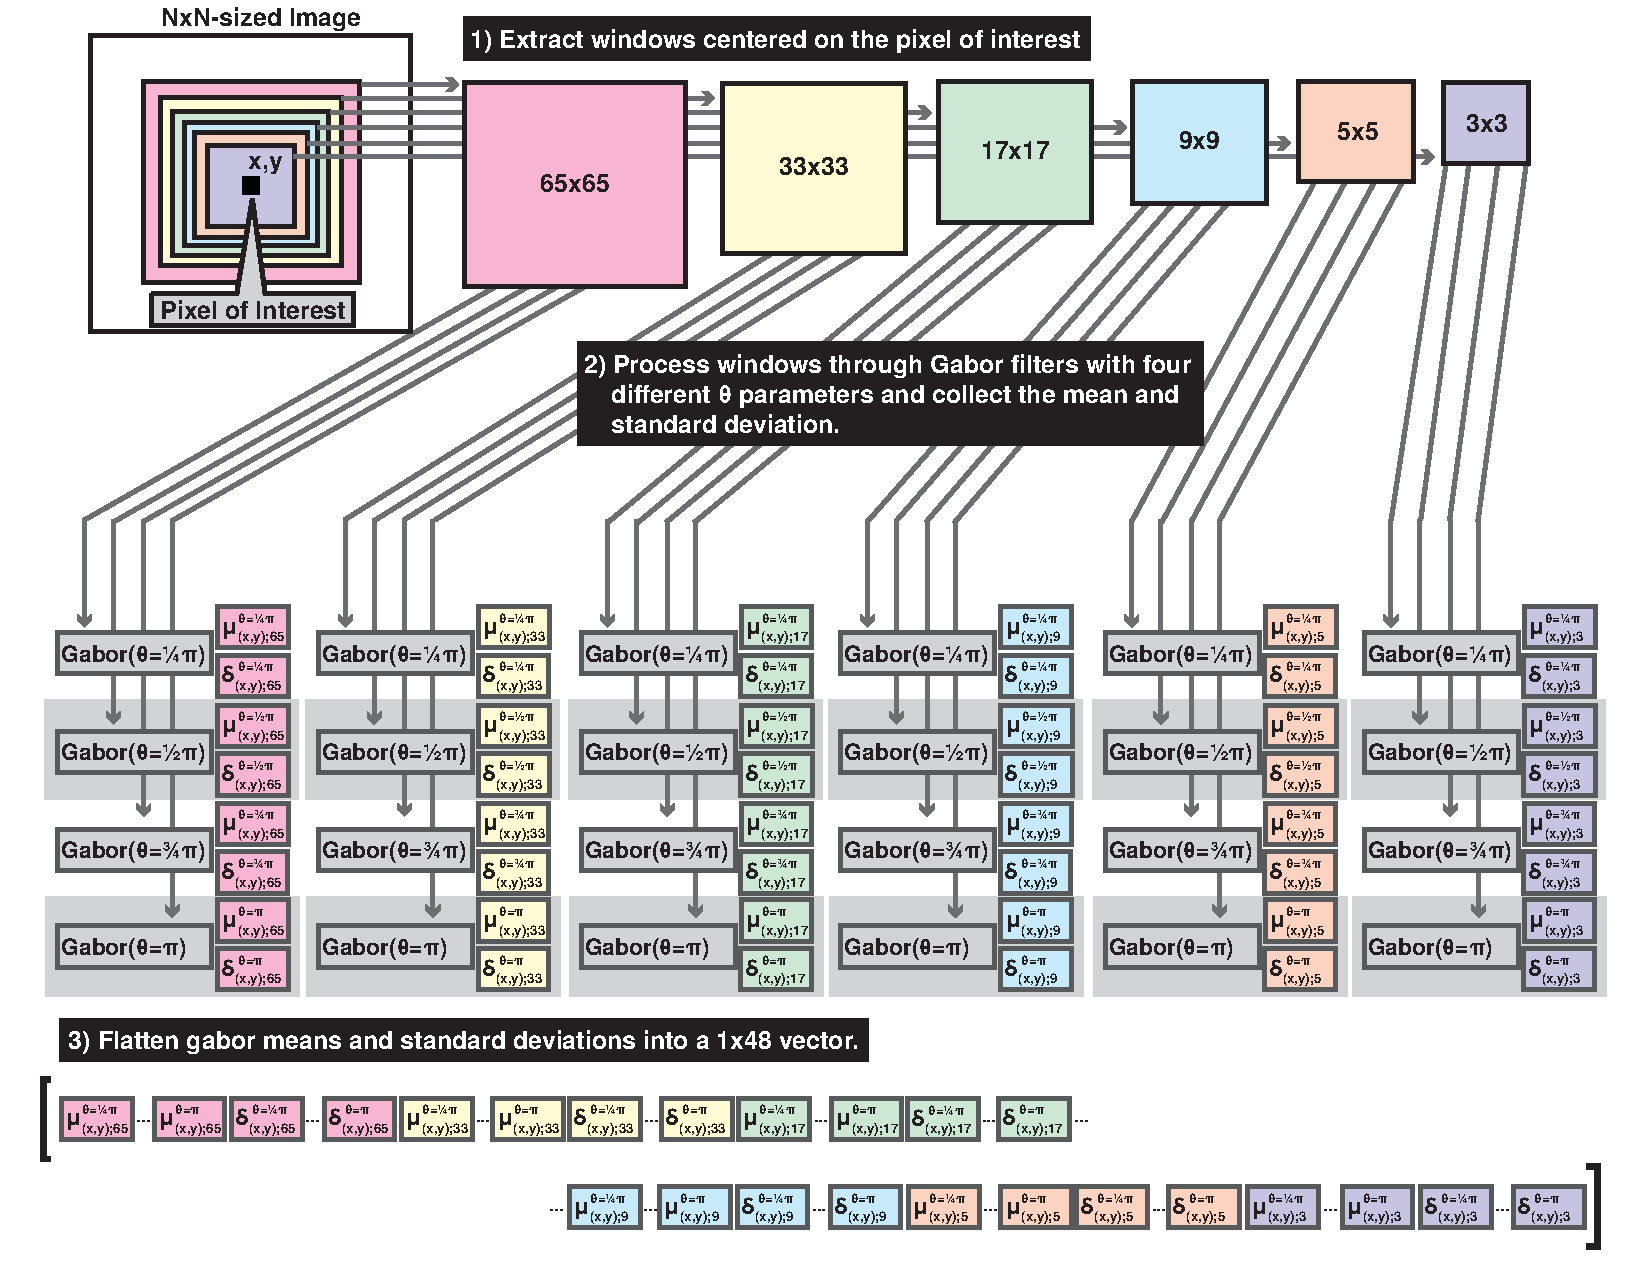
\includegraphics[width=190mm]{figures/gabor-kmknn-figure2.pdf}
		\caption{Diagram illustrating the method by which Gabor features are extracted from images in the PPReCOGG model. \label{gabor_diagram}}
	\end{figure}
\end{landscape}

To reduce computational complexity, images are resized to a resolution of
$256\times256$ pixels. Computation time of training is further reduced by
extracting the features of a randomly sampling of one-quarter of the pixels 
(\emph{i.e.}: For an $N \times N$ image where $N=256$, $\lfloor N^2/4 \rfloor = 16,384$ pixels) from the total population .

\begin{figure}[ht!]
	\centering
	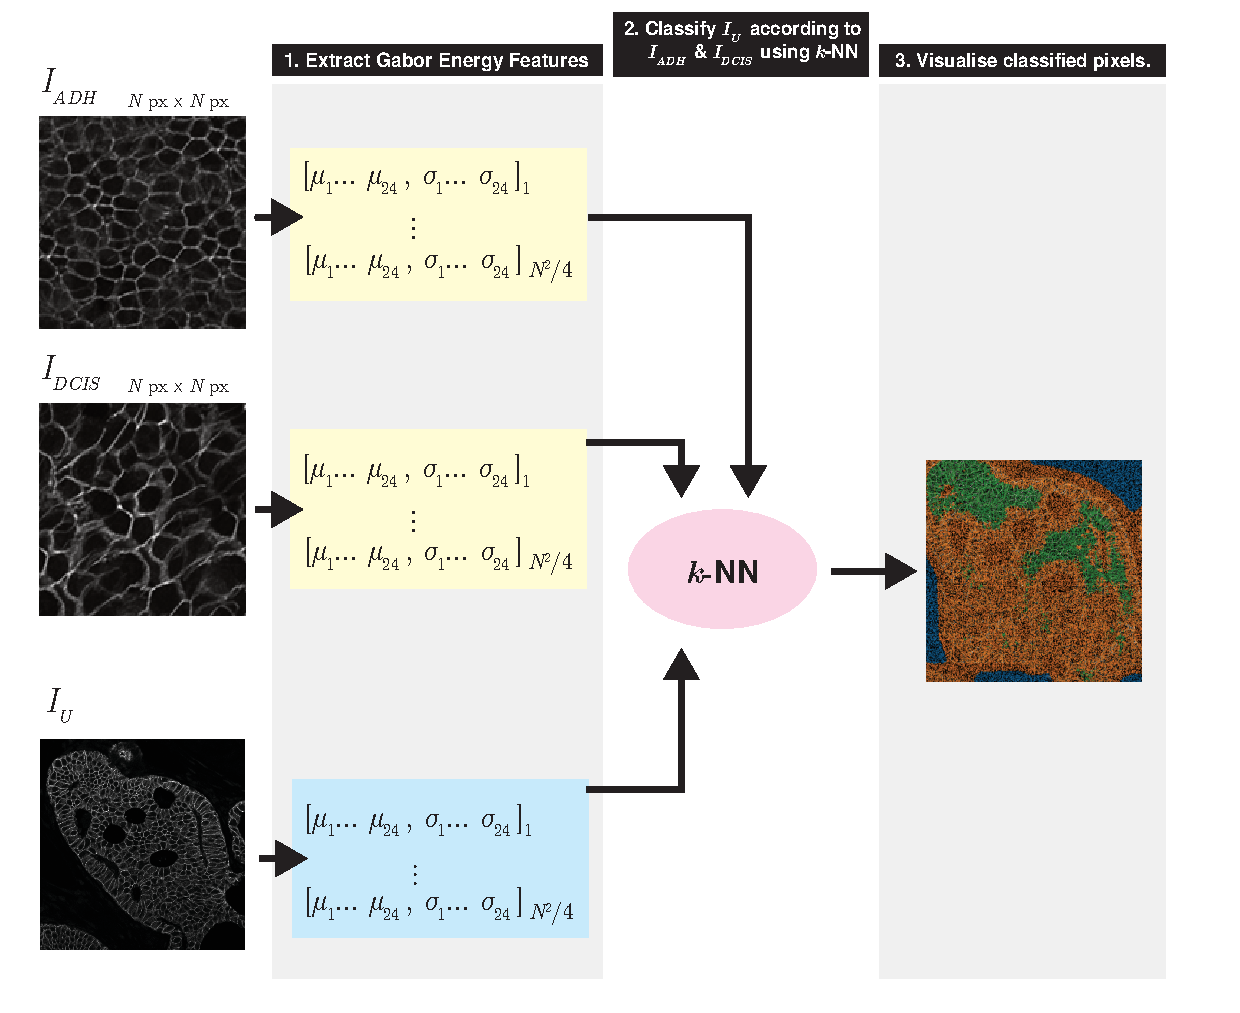
\includegraphics[width=180mm]{figures/pprecogg_summary.pdf}
	\caption{Schematic overview of the PPReCOGG model, wherein Gabor energy features are extracted from images of known classes ($I_{ADH}$, $I_{DCIS}$), as well as an image with regions belonging to different classes ($I_U$). Pixels are classified according to the class of their Gabor energy features, which are classified using the $k$-NN algorithm. \label{pprecogg_summary}}

\end{figure}




%Following the $k$-means for $k$-nearest neighbor
%($k$M$k$NN) model described by Wang 2011, the resultant 48-dimensional
%matrix is clustered using the $k$-means algorithm. The number of
%clusters is determined using the heuristic:

%$$
%k_c = \left \lceil{2\sqrt(n)}\right \rceil
%$$

%Where $k_c$ is the number of clusters to compute, and $n$
%is the number of elements to cluster. If features were computed for all 65,536
%pixels in a $256\times256$ image, a total of 512 clusters would be computed
%$\left(k_c = \left \lceil{2\sqrt(65,536)}\right \rceil = 512\right)$.

%The process of classifying a pixel ($p$) begins by calculating the 48 Gabor
%energy means and standard deviations of $p$ as described above. The nearest
%cluster ($C'$) is determined by choosing the cluster with the minimum Euclidean
%distances between its centroid and the feature vector of $p$. $p$ is then
%classified using the standard $K$-nearest neighbor algorithm with
%feature vectors contained in $C'$ and a $K$-value of 3.

%While the Gabor-kMKNN model was efficient at identifying distinct textures in
%images composed of multiple MeasTex.

